%=========================================================================
% (c) Michal Bidlo, Bohuslav Křena, 2008

\chapter{Úvod}
Nacházíme se v době, kdy už i naše pračky a ledičnky jsou připojeny k internetu a tím pádem s těmito zařízeními můžeme komunikovat vzdáleně. Avšak s přibývajicím počtem zařízení v internetu vyvstává otázka, jak moc jsou tyto  jednotlivé zařízení přístupné i pro nepovolané osoby.
\newline

S totuo problematikou sovisí také to, zda náhodou nemáme v konkrétní síti nějaké zařízení navíc, o kterém bychom nevěděli. 
\newline

Tento článek pojednává a programu \texttt{ISAMON}, který má sloužit pro monitorování sítě a pomoct při již zmiňovaných úskalích, které souvosí s rychle přibývajicmí počtem zařízení v síti.
\newline

V tomto článku však také nalezenete podrobnější informace o technice skenovaní, kterou tento program používá pro zjišťování například všech hostů, kteří jsou připojeni k internetu a nachází se v daném rozpětí sítě (více o tomto tématu v kapitole 2) a taktéž jaké techniky jsou použity pro skenování otevřených portů jak za pomocí protokolu TCP, tak i protokolu UDP (více v kapitole 3).
\newline

Dále je zde popsán způsob práce s tímto programem, a taktéž možné návratové kódy (více v kapitole 4).


\chapter{Hledání zařízení v síti}
Jednou ze základních služeb, která tento program nabízí uživatelům, tak je skenování zadané sítě pro nalezení všech aktivníh hostů, kteří jsou připojeni k internetu.
\newline

Všichni hosti jsou povini implemntovat \texttt{ICMP Echo server} funkci, dle \texttt{RFC 1122}. Tato funkce zajišťuje, že host korektně příjme \texttt{ICMP Echo request} a vygeneruje a pošle korespodnující \texttt{ICMP Echo replay}.\cite{RFC1122}

Jelikož né všechna zařízení respektují toto \texttt{RFC}, bylo nutné  implementovat dva rozdílné způsoby vyhledávání aktivních klientů. Jeden způsob je použit pro vyhledávání aktivních klientů v lokální síti a drůhý způsob pak při vyhledávání klientů ve vzdálené síti, kde vzdálená síť je definována, jako síť ve které není přítomné zařízení, na kterém běží program \texttt{ISAMON}.

\section{Způsob vyhledávání v lokální síti}
Jak již bylo popsáno výše, tak né každé zařízení respektuje implementaci \texttt{ICMP Echo server}, avšak vyhledávání v lokální síti je usnadněno existencí takzvaného \texttt{Adress Resolution Protocol (ARP)}, který zajišťuje překlad \texttt{IPv4} adresy na \texttt{MAC} adresu konkrétního zařízení. Jelikož bez implementace tohoto protokolu, by zařízení nebylo schopné poslat paket na jiné zařízení v síti, ba dokonce ani na směrovač, je tento protokol použit při skenování lokání sítě.
\newline



\subsection{Implementace skenování zařízení v lokání síti}
Skenování je založené na \texttt{ARP}. Na začátku skenování je vygenerován \textit{ethernetový rámec}, který je specifikován v \texttt{RFC 826}\cite{RFC826} a obsahuje konkrétní \texttt{IPv4} adresu hledaného zařízení v síti. Pro odeslání \texttt{ARP} rámce bylo zapotřebí použít takzvaný \textit{RAW socket}. 

Pokud zařízení s konkrétní \texttt{IPv4} adresu existuje v lokální síti, tak je vygenerována patřičná odpověď a program \texttt{ISAMON} tuto odpověď zachytí a přidá \texttt{IPv4} adresu tohoto zařízení do instance třídy \texttt{IsamonLiveVect}, což je speciální vektor, který udržuje informace o aktivních zařízeních ve skenované síti.

Pokud však zařízení v síti neexistuje, program \texttt{ISAMON} žádnou odpověď nezachytí a po vypršení časovače přestane čekat na odpověď a považuje zařízení za neaktivní, tudíž toto zařízení není přidáno do instance třídy \texttt{IsamonLiveVect}, a nebude na něm prováděno případné další skenování.
\newline

Pozn: Při pokoušení se oskenovat sám sebe, není poslán ARP dotaz, protože by byl bezdůvodný (\textit{tzv: Gratuitous}), přičemž by se nevygenerovala patřičná odpoveď a tím pádem by se naše zařízení tvářilo jako by bylo neaktivní. V tomto případě se přistupuje k vlastnímu zařízení jako kdyby toto zařízení bylo ve vzdálení síti, avšak musí se naslouchat na takzvaném \textit{loopback} zařízení.

\section{Způsob vyhledávání ve vzdálené síti}
Zde se nám nabízí jen několik málo různých přístupů k prohledávání vzdálené sítě a jedním z nich je použití protokolu \texttt{Internet Control Message Protocol (ICMP)}, avšak počítá se s tím, že v síti se některé pakety mohou ztratit (tzn. nedorazí k cíli), popřípadě mohou být zahozeny (vypršení TTL), takže tento způsob není vždy dokonalý.

\subsection{Implementace skenování zařízení ve vzdálené síti}
Při začátku skenování tohoto vzdáleného zařízení se na začátku vytvoří paket, dle popisu v \texttt{RFC 792}\cite{RFC792}, tomuto paketu se přenastaví TTL na co nejvyšší hodnotu (konkrétně \textit{255}), aby se předešlo zahazování paketů, a daný sestavený paket se pomocí specifického rozhraní pošle do sítě. 

Pokud zařízení s konkrétní \texttt{IPv4} adresu existuje a taktéž na tomto zařízení je korektně implementován \texttt{ICMP Echo server}, tak  tak vygeneruje patřičnou odpověď (jedná se \textit{ICMP Echo replay}) a tato odpověď je zachycena programem \texttt{ISAMON} a poté zpracována. Výsledkem zpracování je přidání adresy tohoto aktivního zařízení do instance třídy \texttt{IsamonLiveVect}.

Pokud však zařízení v síti neexistuje, nebo na tomto zařízení není korektně implementován \texttt{ICMP Echo server}, program \texttt{ISAMON} žádnou odpověď nezachytí a po vypršení časovače přestane čekat na odpověď a považuje zařízení za neaktivní, tudíž toto zařízení není přidáno do instance třídy \texttt{IsamonLiveVect}, a nebude na něm prováděno případné další skenování.



\chapter{Skenování portů u aktivních zařízení}
Jednou z dalších důležitých služeb, které jsou implementovány v programu \texttt{ISAMON} je možnost skenovat otevřené porty na jednotlivých aktivních zařízeních za pomoci rozdílných protokolů, jako je UDP \cite{RFC768} nebo TCP \cite{RFC793}.

Jelikož přistupování k těmto protokolům je značně odlišné, jsou jednotlivé techniky skenování popsány ve zvláštních kapitolách.

\section{Skenování TCP portů}
Protokol TCP zajišuje \textit{spojení} dvou zařízení, která se nachází v internetové síti a tento protokol garantuje spolehlivé doručování zpráv oběma směry. Na začátku spojení dvou zařízení pomocí tohoto protokolu je vždy takzvaný \textit{TCP handshake} (viz obrázek), který zajišťuje, že o sobě dané dvě zařízení ví a jsou připraveny na vzájemnou komunikaci. 
\newline

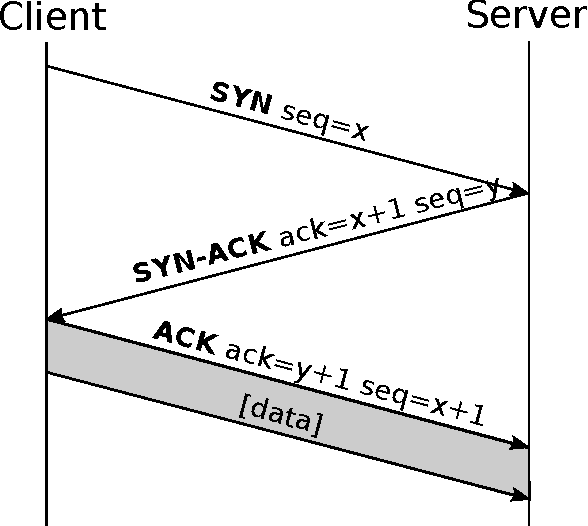
\includegraphics{obrazky-figures/Tcp-handshake.pdf}

Tohoto způsobu je využito i při scenování TCP portů. Na začátku program \texttt{ISAMON} zašle TCP paket s příznakem \textit{SYN} na konkrétní port u aktivního skenovaného hosta a očekává, že příjde paket s nastavenými příznaky buď \textit{SYN-ACK} (v tomto případě je port otevřený), a nebo příjde paket s nastaveným příznakem \textit{RST} (v tomto případě jde o zavřený port).

\subsection{Implemetace skenování TCP portů}
 Na začátku skenování pomocí TCP je otevřen \textit{TCP socket}, kterým zajistíme, že odeslaný paket bude mít formát a strukturu pospanou v \texttt{RFC 793} \cite{RFC793}. 
 
 Dále je nastaveno internetové rozhraní, které bude sloužit pro komunikaci mezi zařízeními. Jelikož požadujeme, aby skenování bylo co nejrychlejší, tak je použit neblokujicí \textit{connect}, který nám dovoluje nečekat na potvrzovací pakety a popřípadě zasílat na jiný port či jiného aktivního hosta další požadavky. 
 
 Příchozí pakety jsou odchytáváný za pomocí aplikačního rzhraní zvaného \textit{libpcap}, které dokáže zpracovávat odchycené pakety. Pokud je tedy odchycen paket, který má nastavený příznak \textit{SYN-ACK}, pak je tento port přidán jako otevřený ke konkrétnímu aktivnímu hostu.

\section{Skenování UDP portů}
Protokol UDP je, oproti TCP protokolu, \textit{nespojovaný} a taktéž nezaručuje doručení paketů. V UDP protokolu neexistuje ani nic jako v TCP \textit{TCP handshake}, který by nás informoval o povedení spojení, či ne. Jediné však co je generované a podel čeho lze usoudit, zda daný UDP port je otevřen, či zavřen, tak je informace ohledně nedostupnosti portu, kde tato informace je přenáčena protokolem \texttt{ICMP} a nazývá se obecně \textit{Port Unreachable}\cite{RFC1122}. Jediný možný způsob tedy je, že jsou odeslána data na dané aktivní zařízení a konkrétní UDP port a čeká se jestli se navrátí \textit{ICMP Port unreachable}, a nebo se nevratí nic.

\subsection{Implemetace skenování UDP portů}
Na začátku skenování pomocí UDP je otevřen \textit{UDP socket}.

Dále je nastaveno internetové rozhraní, které bude sloužit pro komunikaci mezi zařízeními. Poté se již odešle prázdná zpráva s délkou 0 na daný UDP port daného aktivního klienta.

Příchozí pakety jsou odchytáváný za pomocí aplikačního rzhraní zvaného \textit{libpcap}, které dokáže zpracovávat odchycené pakety. Pokud je odchycen \textit{ICMP} packet, jehož \textit{type} a \textit{code} odpovídá \textit{Port unreachable}, pak je zřejmé, že tento port je zavřen.

Avšak pokud do vypršení časovačče nedostaneme odpověď, pak si jen můžeme domyslet, že daný port je otevřen.
\newline

Pozn: Skenování UDP portů je velmi nepřesné a taktž velmi zdlouhavé. V realém nasazení né každý host má naimplementovaný \textit{ICMP Destination port unreachable}, protože tato funkcionalita je pouze doporučená a né přikázaná. Dalším úskalím, které se oběvuje při skenovní UDP portů, tak je omezní počtu poslaných \textit{ICMP} zpráv za jednotku času.



\chapter{Použití programu \texttt{ISAMON}}
Jak lze spouštěť:
\newline
\texttt{isamon [-h] [-i <interfc>] [-t] [-u] [-p <port>] [-w <ms>] -n <net\_addr/mask> }

\texttt{-h -{}-help} $\Rightarrow$ zobrazení nápovědy

\texttt{-i -{}-interface <interface>} $\Rightarrow$ rozhraní na kterém bude nástroj scanovat

\texttt{-n -{}-network <net\_address/mask>} $\Rightarrow$ ip adresa síťe s maskou definující rozsah pro scanování 

\texttt{-t -{}-tcp} $\Rightarrow$ použije TCP 

\texttt{-u -{}-udp} $\Rightarrow$ použije UDP 

\texttt{-p -{}-port <port>} $\Rightarrow$ specifikace scanovaného portu, pokud není zadaný, scanujte celý rozsah

\texttt{-w -{}-wait <ms>} $\Rightarrow$ jak dlouho se bude čekat na odpověď (výchozí nastavení jsou 2 sekundy)
\newline

\section{Příklady použití}
Pár příkladů:

\texttt{\$ isamon -h } $\Rightarrow$ vypíše se nápověda
\newline

\texttt{\$ isamon -i eth0 -n 192.168.1.0/24} 

$\Rightarrow$ provede se scanování sítě a zobrazí se aktivní klienti za použití rozhraní eth0
\newline

\texttt{\$ isamon -n 192.168.1.0/30}

$\Rightarrow$ provede se scanování sítě a zobrazí se aktivní klienti za použití všech rozhraní 
\newline

\texttt{\$ isamon -n 192.168.1.0/28 -t -p 22}

$\Rightarrow$ provede se scanování sítě a zobrazí se aktivní klienti s otevřeným TCP portem 22 za použití všech rozhraní 
\newline

\texttt{\$ isamon -n 192.168.1.0/30 -t -u -w 5}

$\Rightarrow$ provede se scanování sítě a zobrazí se aktivní klienti a všechny otevřené TCP a UDP porty za použití všech rozhraní, pokud klient neodpoví do 5ms, daný port je povaován za uzavřený

\section{Návratové kódy}
Program \texttt{ISAMON} může skončit s těmito návratovými kódy:

	\texttt{0} : Všechno probělo v pořádku
	
	\texttt{1} : CHYBA - v parsování argumentů
	
	\texttt{2} : CHYBA - v nastavení adresy sítě či masky
	\newline
	
	\texttt{5} : CHYBA - způsobená při získávání informací o rozhraních
	
	\texttt{6} : CHYBA - ve vytváření nebo odesílání ICMP packetu
	
	\texttt{7} : CHYBA - při vytváření TCP soketu 
	
	\texttt{8} : CHYBA - při vytváření či odesílání UDP packetu
	\newline
	
	\texttt{10} : CHYBA - při odchytávání packétu (pcap chyba)
	
	




%=========================================================================
